% Created 2020-06-23 火 10:28
\documentclass{article}
\usepackage[utf8]{inputenc}
\usepackage[T1]{fontenc}
\usepackage{fixltx2e}
\usepackage{graphicx}
\usepackage{longtable}
\usepackage{float}
\usepackage{wrapfig}
\usepackage{rotating}
\usepackage[normalem]{ulem}
\usepackage{amsmath}
\usepackage{textcomp}
\usepackage{marvosym}
\usepackage{wasysym}
\usepackage{amssymb}
\usepackage{hyperref}
\tolerance=1000
\usepackage[margin=1.0in]{geometry}
\usepackage{mymacros}
\usepackage{amsmath,amssymb,amsthm}
\author{hisanobu-nakamura}
\date{\textit{<2020-06-18 木>}}
\title{Inversion of conics}
\hypersetup{
  pdfkeywords={},
  pdfsubject={},
  pdfcreator={Emacs 25.3.2 (Org mode 8.2.10)}}
\begin{document}

\maketitle
Title: Inversion of conics
Date: 2020-06-18
Category: math
Tags: math


\section{Inversion}
\label{sec-1}
The images of lines and circles under inversion in circles are again circles and lines.
 This is the well-known fact of the inversion geometry.
 But somewhat less known fact about the inversion in circles is that quadratic curves are inversed into certain types of famous quartic curves which have been known from antiguity.
 In general, the image of a real algebraic curve of degree n, $F(x,y)=0$ under inversion in unit circle at the origin satisfies an equation $F(\frac{x}{R^2},\frac{y}{R^2}) = 0$,
 where $R = \sqrt{x^2 + y^2}$, which is an algebraic expression of degree $2n$.
 Here we will see how the quadratic curves or conics are mapped under this transformation.
\section{Inversions of conics}
\label{sec-2}
\subsection{Hyperbola}
\label{sec-2-1}
Rectagular hyperbola
\begin{equation}
\label{ }
x^2 - y^2 = 1
\end{equation}
maps to the Bernouilli's lemniscate
\begin{equation}
\label{ }
(x^2 + y^2)^2 = x^2 - y^2.
\end{equation}

\begin{figure}[htb]
\centering
\includegraphics[width=70mm]{./images/hyperbola-lemniscate-pair.png}
\caption{\label{fig:inv-rec-hyp}Inversion of the rectangular hyperbola $x^2 -y^2 = 1$.}
\end{figure} \\

\begin{figure}[htb]
\centering
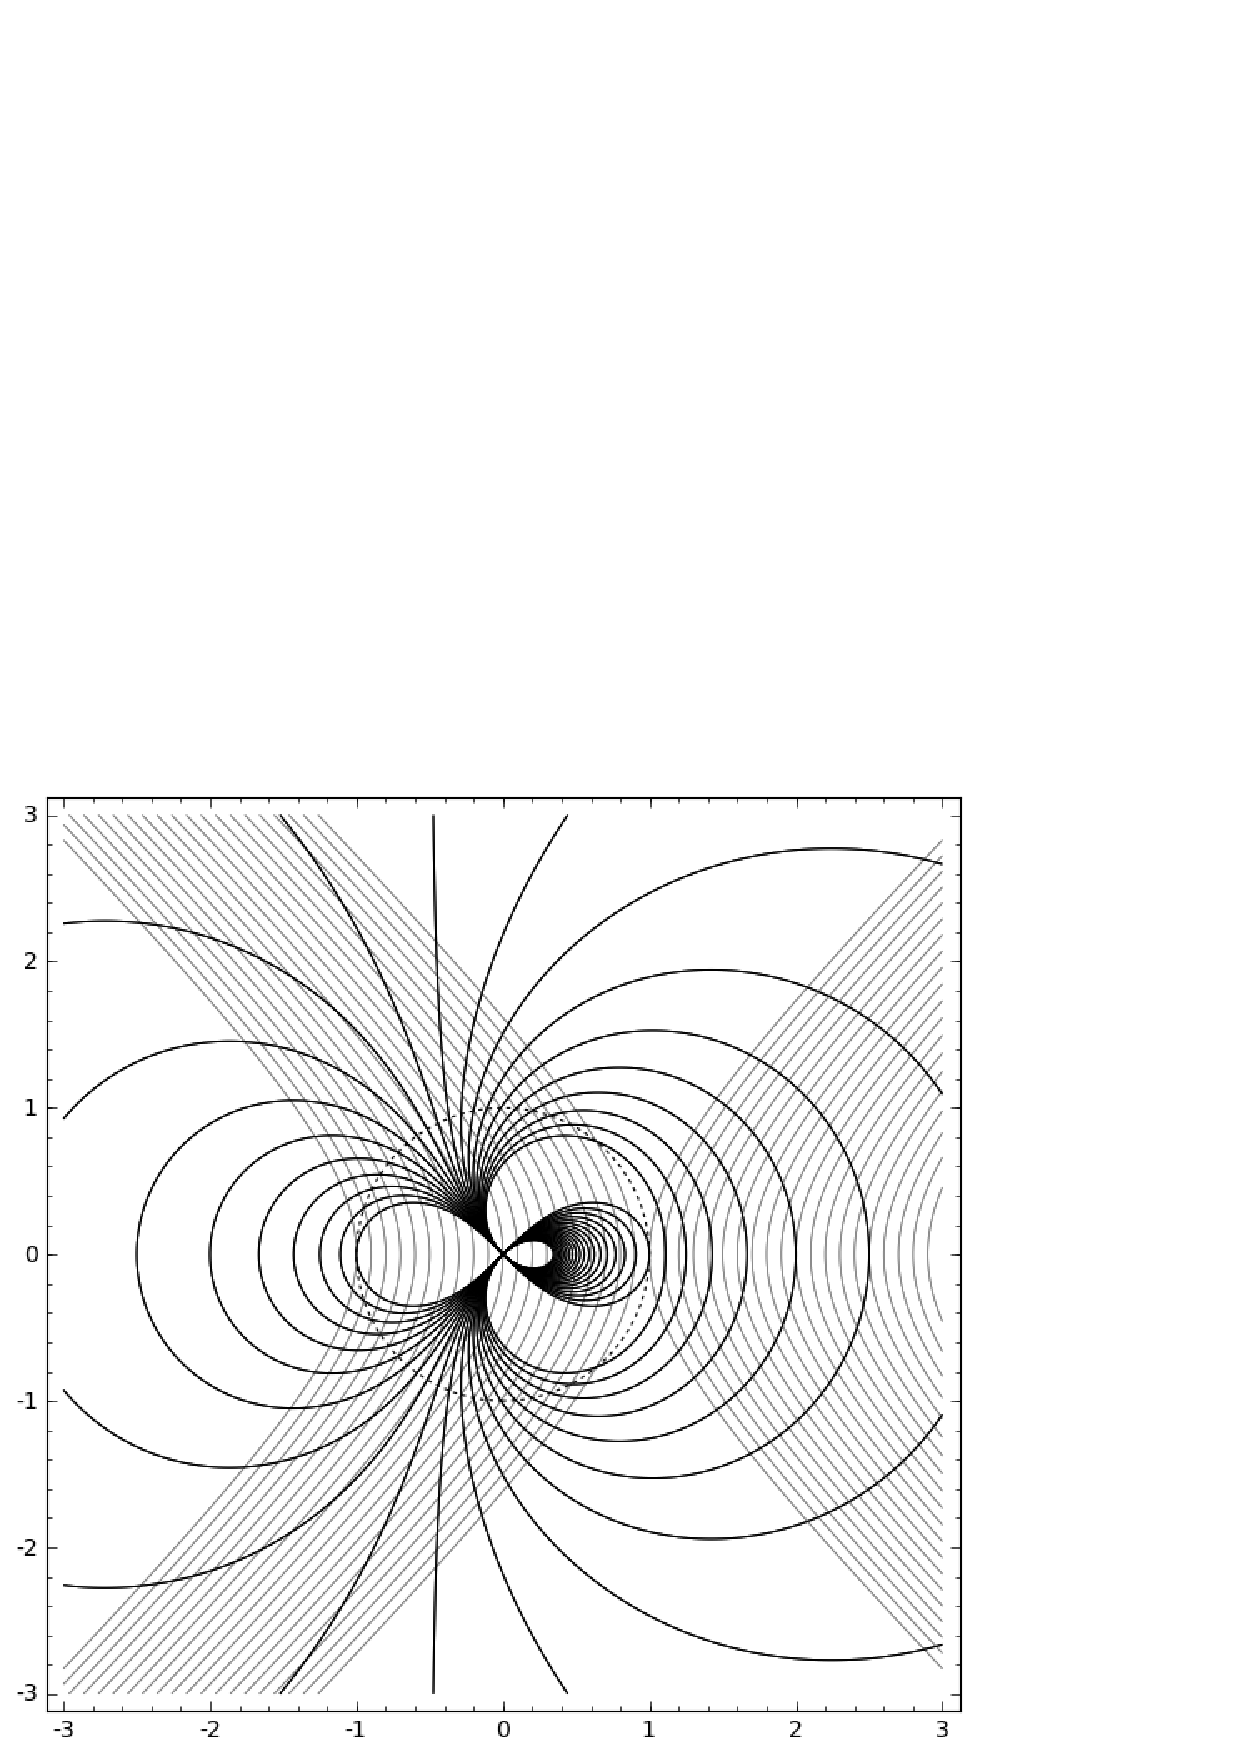
\includegraphics[width=70mm]{./images/hyperbola_locus.png}
\caption{\label{fig:}Inversive images of $(x-a)^2 -y^2 = 1$ with varying $a$}
\end{figure}

\subsection{Parabola}
\label{sec-2-2}

\begin{equation}
\label{ }
y^2 + 1 = x
\end{equation}
maps to a droplet-like curve
\begin{equation}
\label{ }
y^2 + (x^2 + y^2)^2 = x(x^2 + y^2).
\end{equation}

\begin{figure}[htb]
\centering
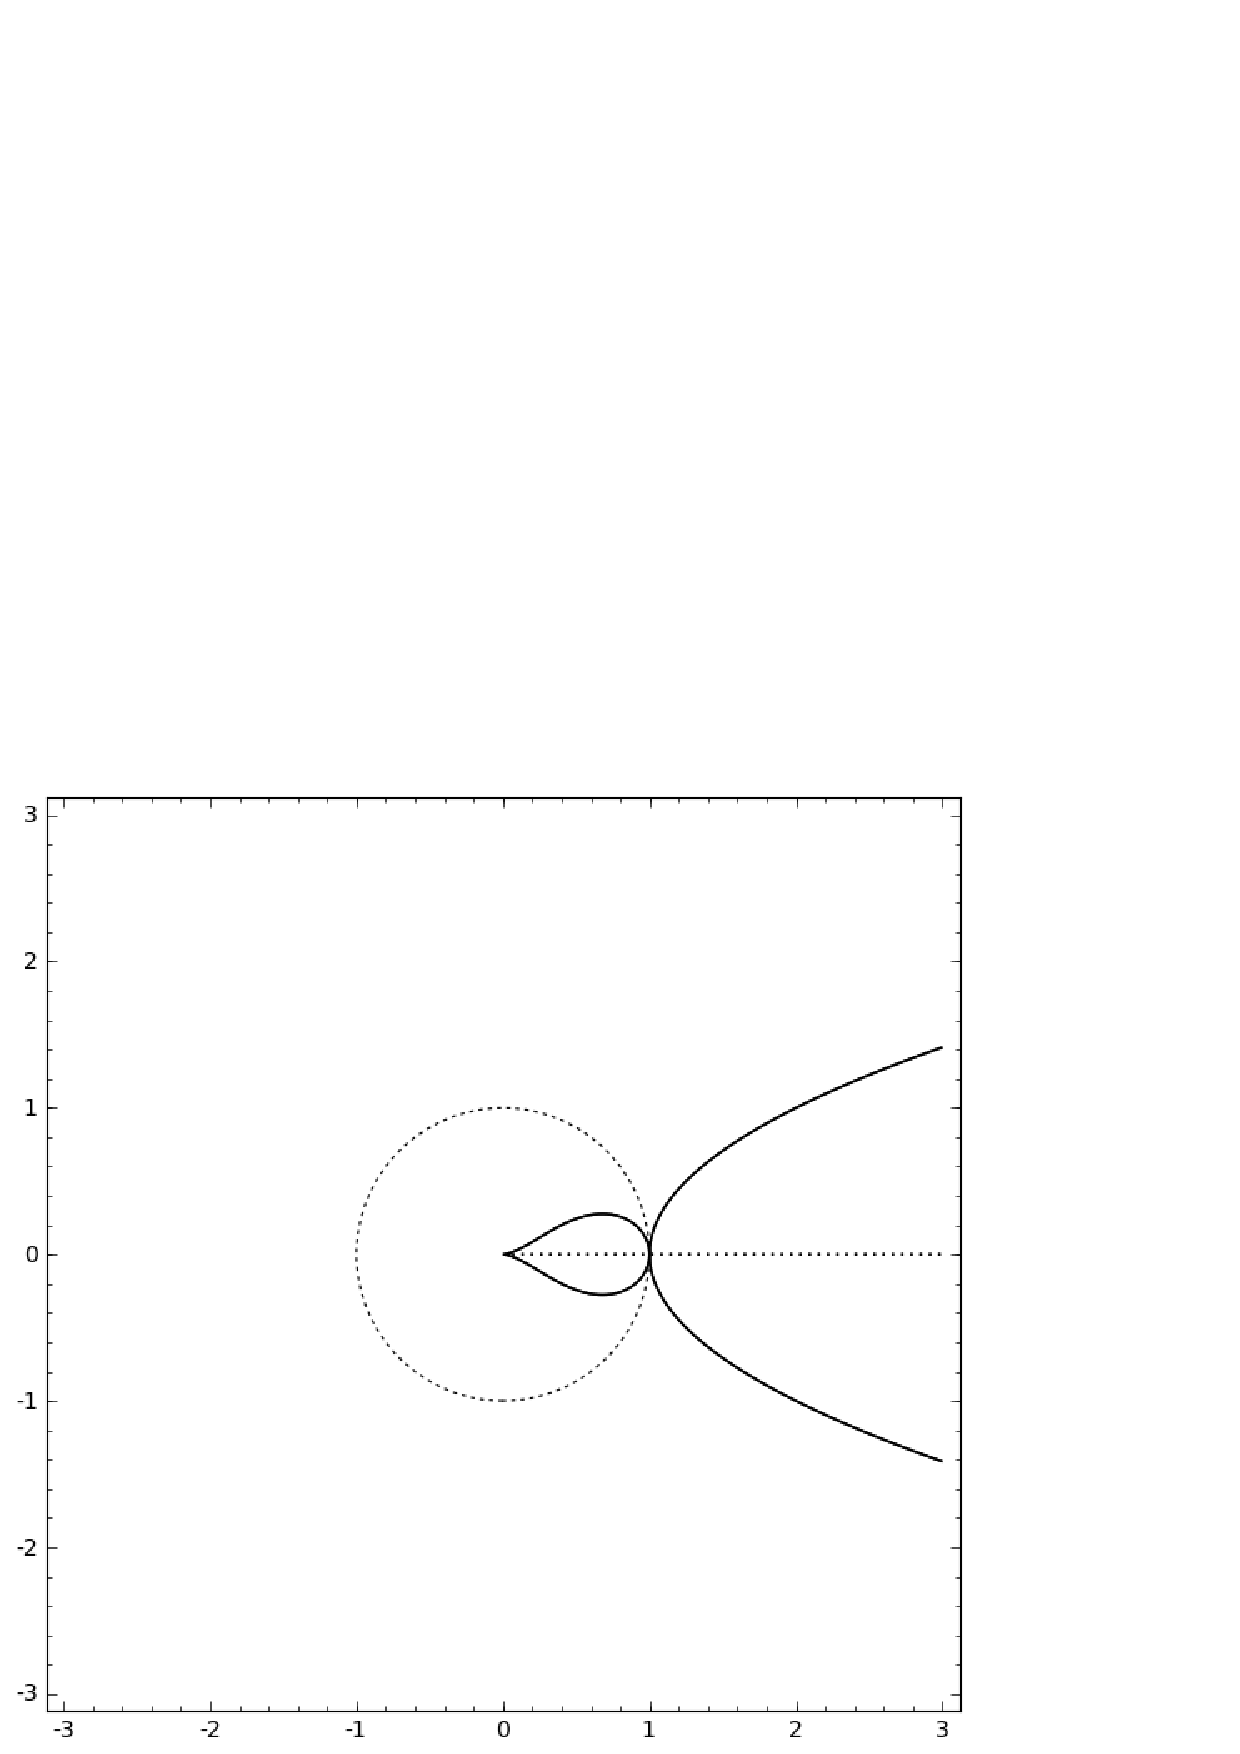
\includegraphics[width=70mm]{./images/para_drop.png}
\caption{\label{fig:para-drop}Inversion of parabola $y^2+1=x$}
\end{figure}

\begin{figure}[htb]
\centering
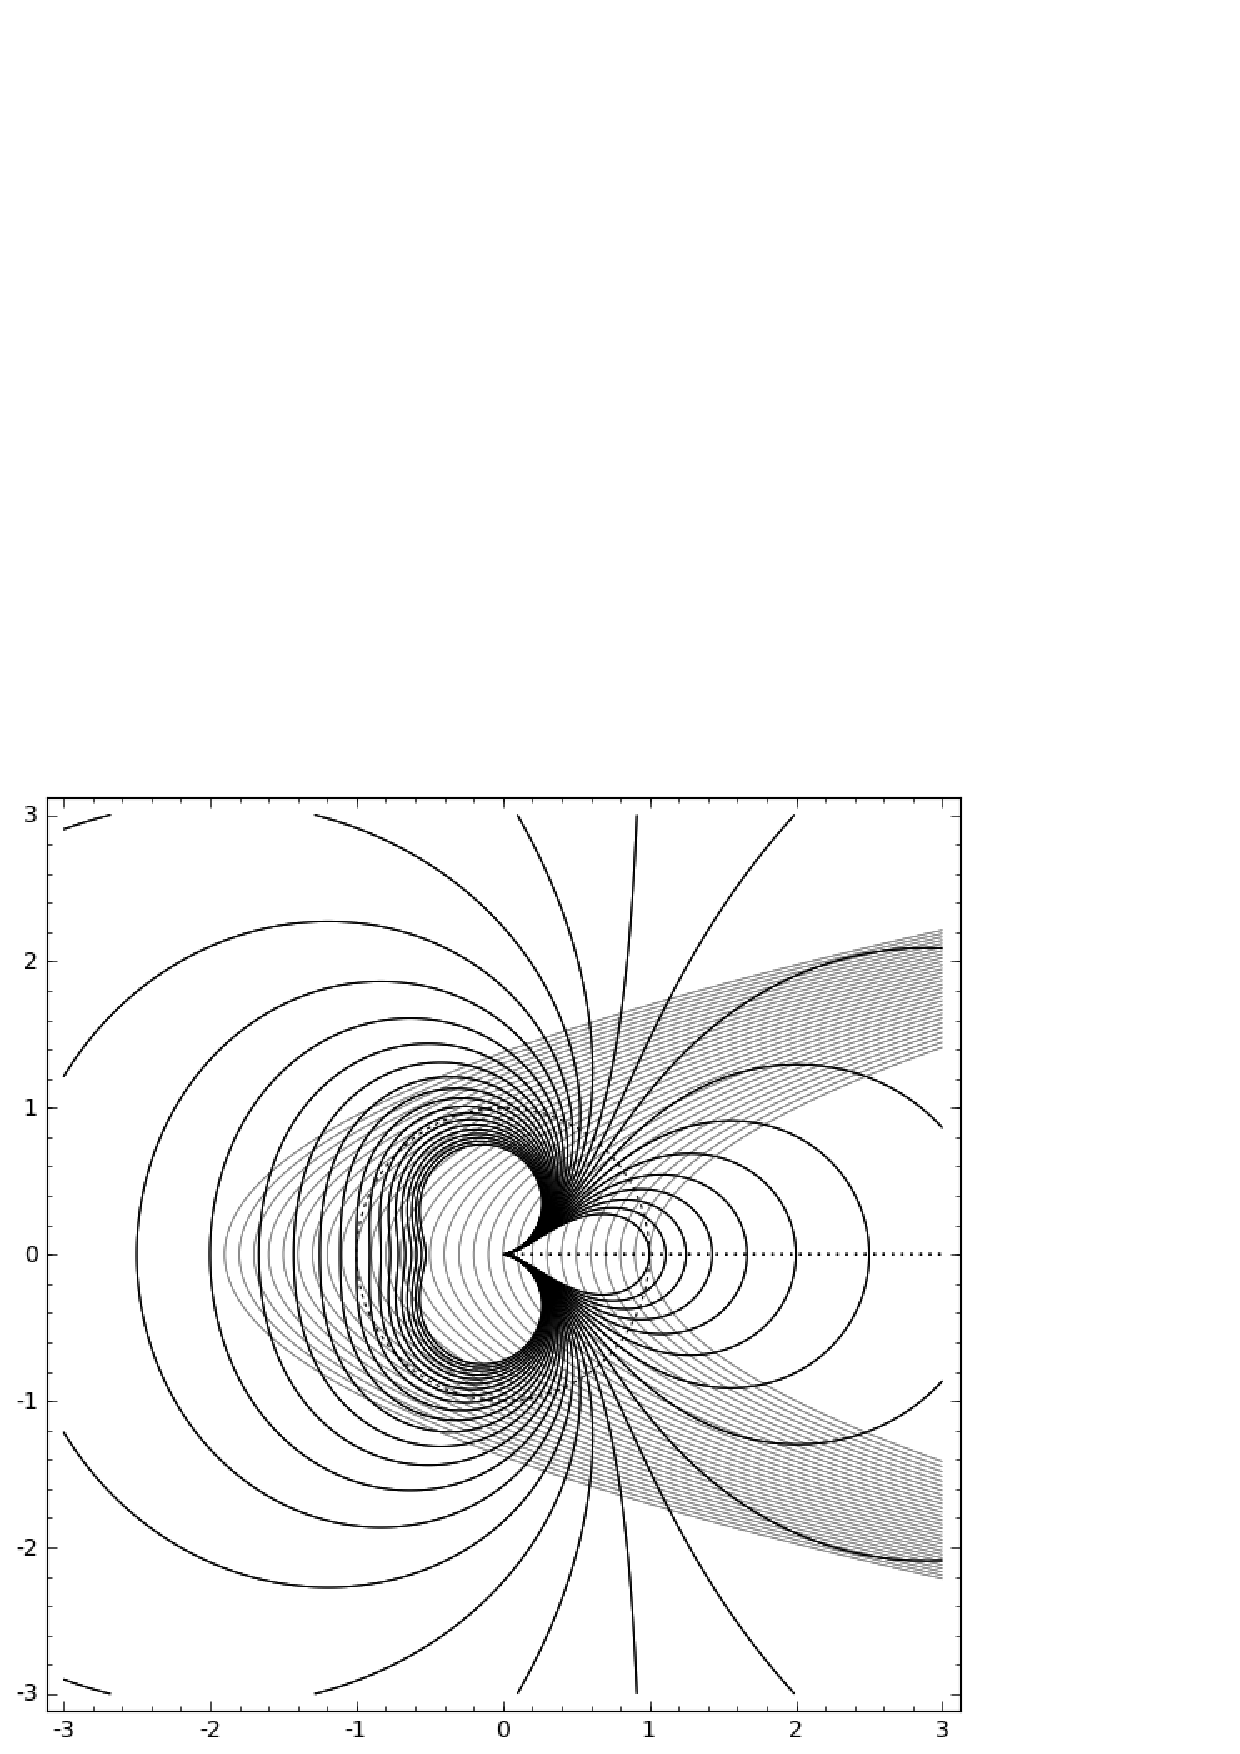
\includegraphics[width=70mm]{./images/parabola_locus.png}
\caption{\label{fig:}Inversive images of $y^2 = x-a$ with varying $a$}
\end{figure}

\subsection{Ellipse}
\label{sec-2-3}
\begin{equation}
\label{ }
\frac{x^2}{a^2} + \frac{y^2}{b^2} =1
\end{equation}
maps to a hippopede
\begin{equation}
\label{ }
(x^2 + y^2)^2 = A^2x^2 + B^2 y^2.
\end{equation}

\begin{figure}[htb]
\centering
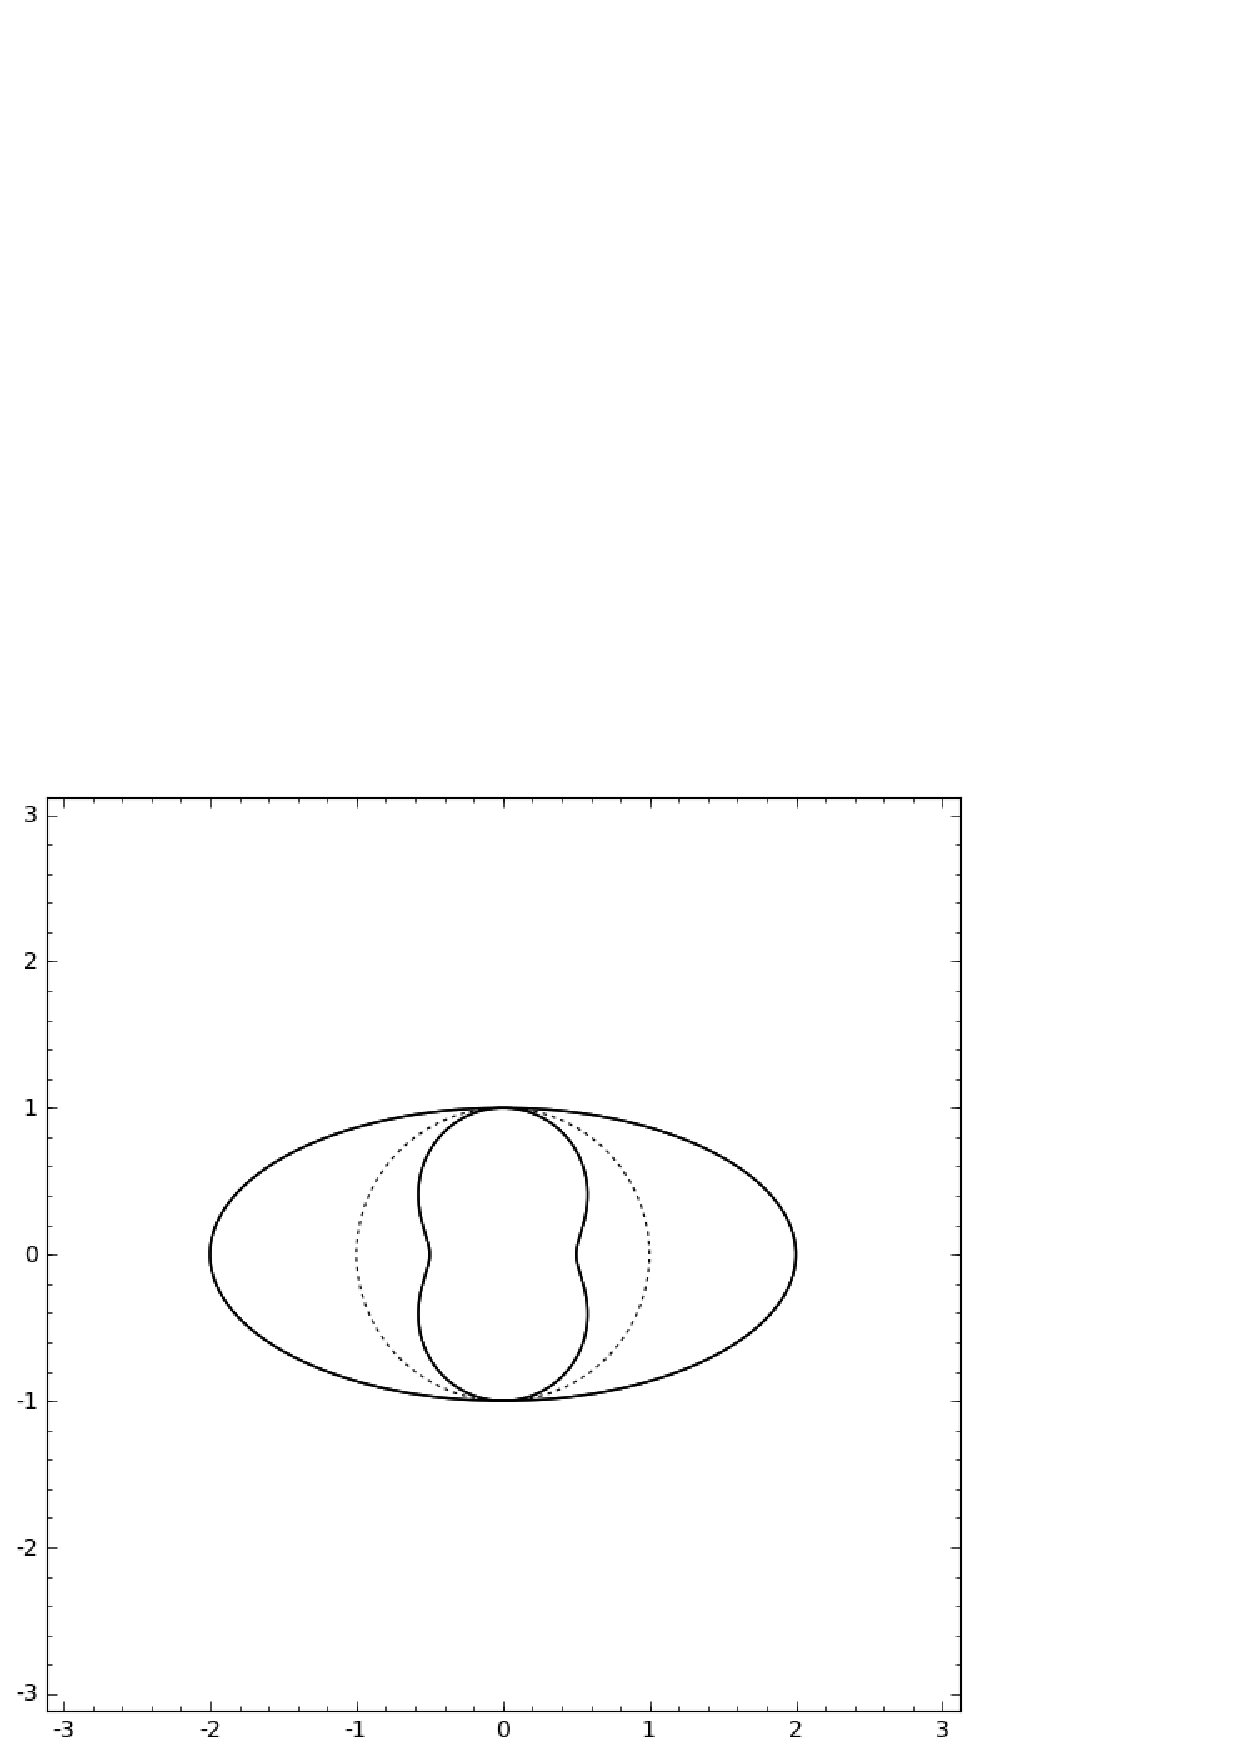
\includegraphics[width=70mm]{./images/ell_vase.png}
\caption{\label{fig:para-drop}Inversion of ellipse $\frac{x^2}{4}+y^2 = 1$}
\end{figure}

\begin{figure}[htb]
\centering
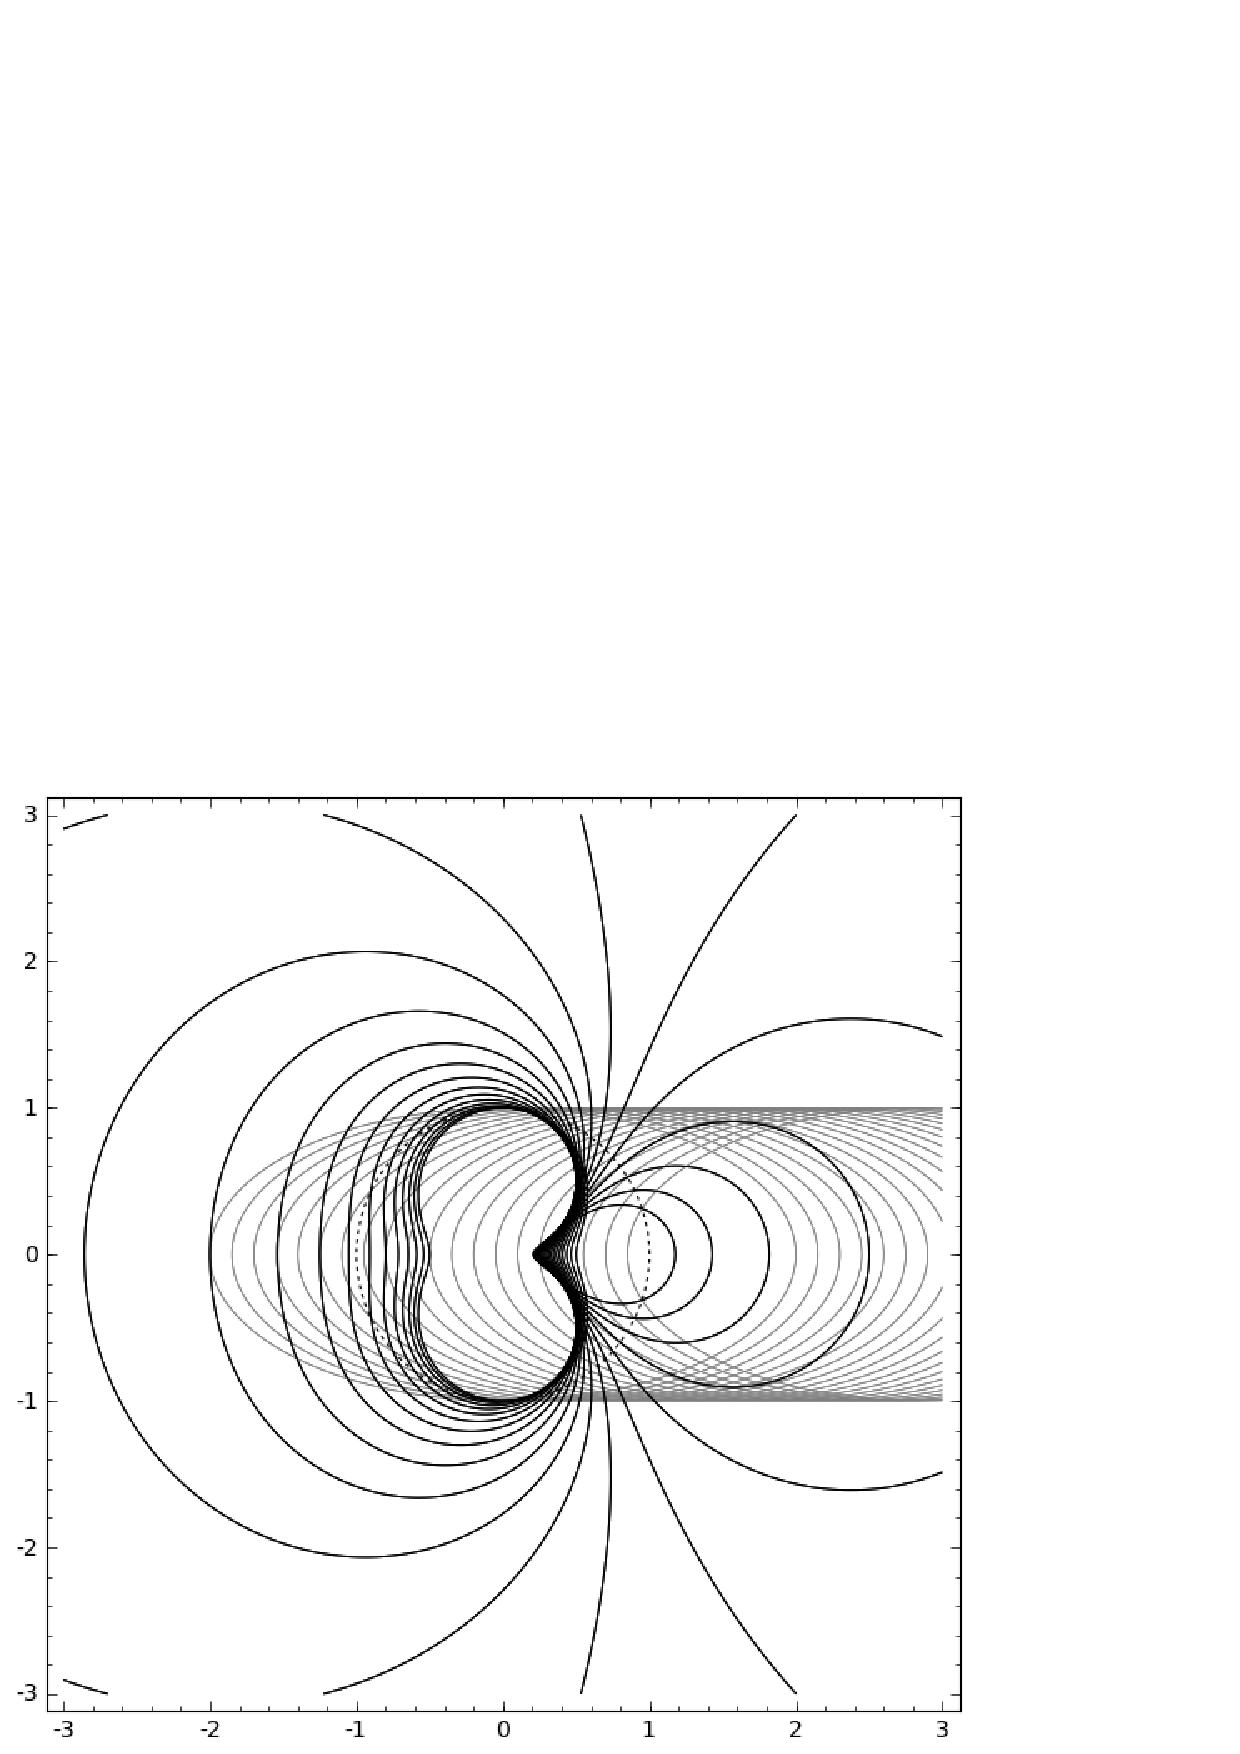
\includegraphics[width=70mm]{./images/ellipse_locus.png}
\caption{\label{fig:}Inversive images of $\frac{(x-c)^2}{a^2} -\frac{y^2}{b^2} = 1$ with varying $c$}
\end{figure}
% Emacs 25.3.2 (Org mode 8.2.10)
\end{document}